\section{Testing}

Das testen der Anwendung stellte uns zu Anfang vor einige Probleme die es zu lösen galt. Zum Beispiel wie können wir die Frequenz eines Erbebens simulieren, wie genau reagieren die Sensoren von verschiedenen Geräten auf das Erdbeben, bestehen Anzeigeprobleme auf den verschiedenen Displaygrößen, wie sieht die Darstellung auf dem Tablet aus, wie stark beeinflusst die Performance der Geräte die Messung bzw. das Benutzererlebnis und nicht zuletzt wie hoch ist der Akkuverbrauch wenn die App im Hintergrund läuft.

\subsection{Lösungsansätze}

Zum lösen des Problems der Simulation eines Erbebens fielen uns folgende Ansätze ein:

\begin{itemize}
	\item Eine Rüttelplatte auf der die Geräte liegen
	\item Schütteln der Geräte bis sie auslösen
	\item Klopfen direkt auf das Gerät bzw. auf den Tisch neben dem Gerät
\end{itemize}

Zur Anpassung der Sensoren von verschiedenen Geräten könnte man die Frequenz der Messung so anpassen das im Mittel alle Geräte auslösen wenn sie zusammen auf einer Fläche liegen an der Gerüttelt wird. Eine weitere Möglichkeit wäre die Geräte zu Schütteln bis sie auslösen hierbei besteht aber das Problem das die Frequenz beim nacheinander schütteln der Geräte nicht exakt die gleiche wäre.\\

Zum Messen ob die Performance des Gerätes sich auf die Darstellung in der App auswirkt gibt es Apps die die aktuelle Framerate anzeigen oder als andere Möglichkeit kann man sich auf sein subjektives Gefühl verlassen ob die App flüssig läuft.\\

Den Akkuverbrauch könnte man entweder mit einem extra hierfür programmierten Tool genau messen oder mit den Bordmitteln von Android ungefähr bestimmen was aber nicht so genau wäre.\\

\subsection{Durchführung} 

Zur Durchführung der Tests haben wir verschiedene Geräte eingesetzt hier eine Auflistung der Geräte mit ihren Spezifikationen.

\begin{figure}[H]
\centering
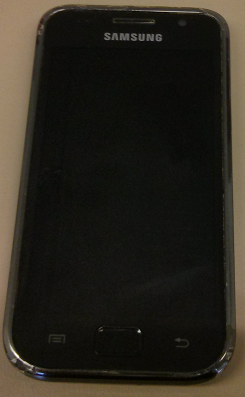
\includegraphics{/galaxys.png}
\caption{Galaxy S}
\label{fig:galaxy S}
\end{figure}

Das Erste Gerät ist ein Samsung Galaxy S aus dem Jahr 2010 es besitzt einen 1Ghz Singlecore Prozessor und 512Mb RAM das Betriebssystem ist Android 4.4 als CustomROM.\\

\begin{figure}[H]
\centering
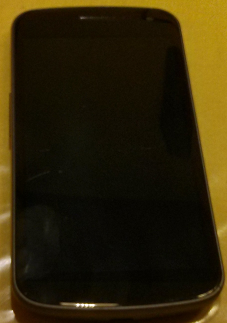
\includegraphics{/galaxynex.png}
\caption{Galaxy Nexus}
\label{fig:galaxynex}
\end{figure}

Das Zweite Gerät ist ein Google Galaxy Nexus aus dem Jahr 2011 es besitzt einen 1,2Ghz Dualcore Prozessor und 1Gb RAM das Betriebssystem ist Android 4.3.\\

\begin{figure}[H]
\centering
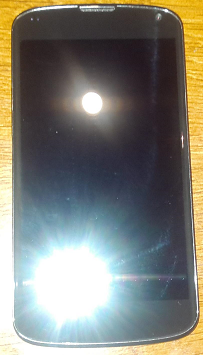
\includegraphics{/nexus4.png}
\caption{Nexus 4}
\label{fig:nexus4}
\end{figure}

Das Dritte Gerät ist ein Google Nexus 4 aus dem Jahr 2012 es besitzt einen 1,5Ghz Quadcore Prozessor mit 2Gb RAM das Betriebssystem  ist Android 4.4.\\

\begin{figure}[H]
\centering
\includegraphics{/a500.png}
\caption{Acer Iconia A500}
\label{fig:a500}
\end{figure}

Das Vierte Gerät ist ein Tablet der Firma Acer aus dem Jahr 2011 mit einem 1Ghz Dualcore Prozessor und 1Gb RAM das Betriebssystem ist Android 4.1 als CustomROM.\\

\begin{figure}[H]
\centering
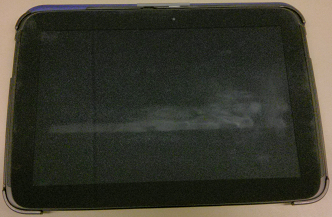
\includegraphics{/nexus10.png}
\caption{Nexus 10}
\label{fig:nexus10}
\end{figure}

Das fünfte Gerät ist ein Google Nexus 10 Tablet aus dem Jahr 2012 mit einem 1,7 Ghz Dualcore Prozessor und 2Gb RAM das Betriebssystem ist Android 4.4\\

Mit dieser Auswahl an Geräten lässt sich die aktuelle verteilung der Android Geräte sowol von der Leistung sowie auch von der Performance gut abbilden. Bei den Tests stellte sich anfangs schnell heraus das die aktualisierungsrate des Graphen in der Appansicht zu hoch war und dieser auf den schwächeren Geräten nicht mehr Flüssig dargestellt werden konnte.\\
Überraschender  weise waren hingegen die Sensordaten der verschiedenen verbauten Beschleunigungssensoren nicht so stark abweichend. Die gröste Abweichung wurde durch ein Bumpercase verursacht das die Vibrationen zu stark abdämpfte. Ansonsten führte die eingestellte Frequenz von Anfang an zu recht passablen Erkennungsraten.\\
Des Weiteren musste die Darstellung auf den verschiedenen Displaygrößen getestet werden hierbei wurde festgestellt das auf Tablets der Raum absolut nicht ausgenutzt wurde hier wurde auf diese Feststellung hin mit der zusätzlichen Entwicklung einer extra Tablet Oberfläche reagiert.\\
Zum Testen der Alarmauslösung benutzen wir am Anfang die einfache Methode indem wir die Geräte solange schüttelten bis sie einen Alarm auslösten. Später haben wir sie auf einen Tisch gelegt und an diesem gerüttelt als einfachen Ersatz für eine Rüttelplatte.\\
Im Späteren Verlauf des Projekts mussten wir außerdem das Auslösen der Alarme durch den Server testen hierzu sprachen wir uns über Whatsapp ab wann wir die Geräte Schütteln müssen und konnten somit auch die Prozentuale Schwelle die im Server implementiert ist testen.\\
des Weiteren waren wir durch unsere Tests immer bemüht den Akkuverbrauch der App zu analysieren und zu optimieren. Hierzu beobachteten wir den Verlauf der Akkubenutzung anfangs mit GPS Ortung ständig aktiviert dieser war viel zu hoch und der Akku innerhalb weniger Stunden komplett entleert. Als nächste Option testeten wir mit einem GPS Aktualisierungsintervall hier waren die Ergebnisse um einiges besser aber immer noch der Akkuverbrauch zu hoch. Als letzte Optimierung testeten wir einen Aktualisierungsintervall der nur im Notfall auf GPS zurückgriff ansonsten aber die anderen Positionsbestimmungsmethoden wie Netz und WLAN nutzte. Hiermit war der Akkuverbrauch in passablen Bereichen und nur auf dem Land etwas erhöht da hier die Position über das Handynetz betimmt wurde und somit teilweise über 3km ungenauigkeit aufwies und deshalb GPS genutzt wurde.\\
\\
Insgesamt sind die Tests gut verlaufen und brachten recht schnell gute Ergebnisse und bei Problemen beim Testen wurde immer schnell auf Verbesserungsvorschläge in der APP sowie im Webservice reagiert. Die Zusammenarbeit bei den Tests war sehr gut.